%\section{$* \rightarrow \omega$}

\subsection{Language Operators: Transformation of $*$-languages to $\omega$-languages}

We already introduced $\lim$. We can define a family of language operators, partly also derived from the study of $\LangOreg$. Some of these operators operate on a single language and not on the class. Let $\Lang$ be a $*$-language class. Let $L \in \Lang$.

We define the following operators on languages, i.e. $\Power(\Sigma^*) \rightarrow \Power(\Sigma^\omega)$:
\begin{enumerate}
\item $\ext(L) := \Set{\alpha \in \Sigma^\omega}{ \exists n \colon \alpha[0,n] \in L} = L \cdot \Sigma^\omega$
\item $\dext(L) := \Set{\alpha \in \Sigma^\omega}{ \forall n \colon \alpha[0,n] \in L}$ (also called the dual-ext)
\item $\lim(L) := \Set{ \alpha \in \Sigma^\omega }{ \forall N \colon \exists n > N \colon \alpha[0,n] \in L } = \Set{ \alpha \in \Sigma^\omega }{ \exists^\omega n \colon \alpha[0,n] \in L }$
\item $\dlim(L) := \Set{ \alpha \in \Sigma^\omega }{ \exists N \colon \forall n > N \colon \alpha[0,n] \in L }$ (also called dual-lim)
\end{enumerate}

From these, we get operators on language classes ($\Power(\Power(\Sigma^*)) \rightarrow \Power(\Power(\Sigma^\omega))$) in a canonical way:
\begin{enumerate}
\item $\ext(\Lang) := \Set{\lim L}{L \in \Lang}$
\item $\dext(\Lang) := \Set{\dext L}{L \in \Lang}$
\item $\lim(\Lang) := \Set{\lim L}{L \in \Lang}$
\item $\dlim(\Lang) := \Set{\dlim L}{L \in \Lang}$
\end{enumerate}

Note that we sometimes combine those operators via union or intersection, e.g. $\ext \cup \dext \Lang := \ext \Lang \cup \dext \Lang$ or $\ext \cup \lim \Lang := \ext \Lang \cup \lim \Lang$. In many cases, it is also interesting to look at boolean combinations of $\omega$-language classes, i.e.:
\begin{enumerate}
\item $\BC \ext \Lang = \BC (\ext (\Lang))$
\item $\BC \lim \Lang = \BC (\lim (\Lang))$
\end{enumerate}

In addition, from historical reasons, we also have the following other language class operators:
\begin{enumerate}
\item $\displaystyle \Kleene(\Lang) := \Set{ \bigcup_{i=1}^n U_i \cdot V_i^\omega}{U_i, V_i \subseteq \Sigma^*, U_i \cdot V_i^* \in \Lang, n \in \N_0}$
\item $\displaystyle \limClosure(\Lang) := \Set{\bigcup_{i=1}^n U_i \cdot \lim V_i}{U_i, V_i \subseteq \Sigma^*, U_i \cdot V_i^* \in \Lang, n \in \N_0}$
\end{enumerate}
In \cref{reg-omega-lang}, we have seen that
\[ \BC \lim \Langreg = \Kleene \Langreg = \limClosure \Langreg . \]

We mostly concentrate on $\ext$, $\lim$ and boolean combinations of them in the rest of this thesis.

For $\ext$ and $\dext$, we can also introduce equivalent $\omega$ automata acceptance conditions (as in \cite{InfCompR101}). Let $L \subseteq \Sigma^*$ be a regular $*$-language and $\A = (Q, \Sigma, q_0, \Delta, F)$ be an automaton which accepts exactly $L$. Let $\alpha \in \Sigma^\omega$. Then
\begin{itemize}
\item $\A$ \defword{E-accepts} $\alpha \ \ \ :\Leftrightarrow \ \ \ \exists \ \text{infinite run $\rho$ in $\A$ which matches $\alpha$} \colon \exists i \colon \rho[i] \in F$,
\item $\A$ \defword{A-accepts} $\alpha \ \ \ :\Leftrightarrow \ \ \ \exists \ \text{infinite run $\rho$ in $\A$ which matches $\alpha$} \colon \forall i \colon \rho[i] \in F$.
\end{itemize}
We define
\begin{itemize}
\item[] $L^\omega_E(\A) := \Set{\alpha \in \Sigma^\omega}{\text{$\alpha$ is E-accepted in $\A$}}$,
\item[] $L^\omega_A(\A) := \Set{\alpha \in \Sigma^\omega}{\text{$\alpha$ is A-accepted in $\A$}}$,
\end{itemize}
and we have the equalities
\begin{itemize}
\item[] $L^\omega_E(\A) = \ext(L)$,
\item[] $L^\omega_A(\A) = \dext(L)$.
\end{itemize}
Note that $\A$ can be both deterministic or non-deterministic for this property (see \cref{gen:e-determinism}).

\

Given these language operators, we are interested in the relations between them. For the class $\Langreg$ of regular languages, we already know that
\[ \LangOreg = \Kleene(\Langreg) = \BC \lim (\Langreg) = \limClosure(\Langreg) . \]

\subsection{Classification of regular $\omega$-languages} %$\Langreg$

\label{regomega-diagram}
Considering $\mathcal{R} := \Langreg$, we get the following language diagram:

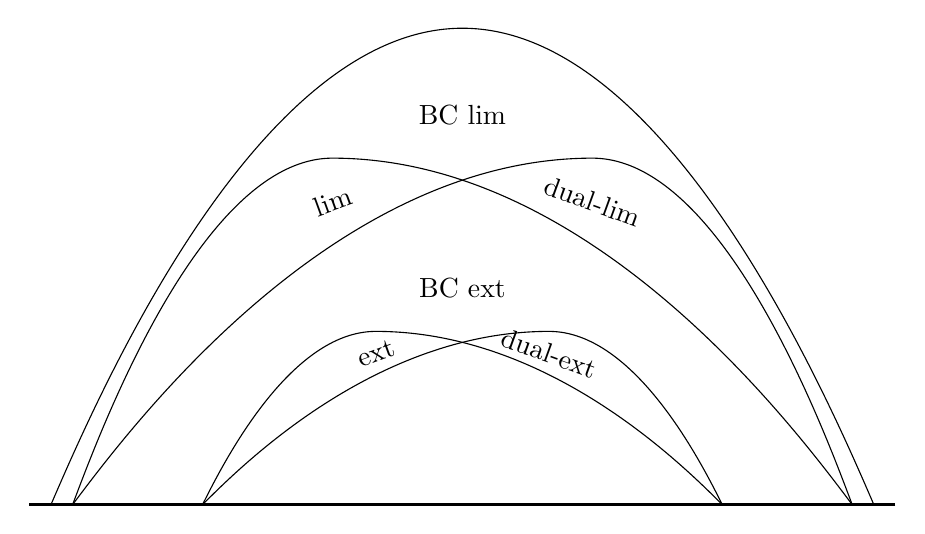
\begin{tikzpicture}
\pgftransformscale{.55}

% http://www.texample.net/tikz/examples/complexity-classes/

%%% HELP LINES - uncomment to design/extend
% \draw[step=1cm,gray,very thin] (-10,0) grid (10,12);
% \node at (0,0) {\textbf{(0,0)}};

%% Horizontal bar
\draw[very thick] (10,0) -- (-10,0);

% BC lim
\draw (-9.5,0) parabola bend (0,11) (9.5,0);
\node at (0,9) {BC lim};

% lim
\draw (-9,0) parabola bend (-3,8) (9,0);
\node[rotate=20] at (-3,7) {lim};

% dual-lim
\draw (-9,0) parabola bend (3,8) (9,0);
\node[rotate=-20] at (3,7) {dual-lim};

% BC ext
%\draw (-6.5,0) parabola bend (0,6) (6.5,0);
\node at (0,5) {BC ext};

% ext
\draw (-6,0) parabola bend (-2,4) (6,0);
\node[rotate=20] at (-2,3.5) {ext};

% dual-ext
\draw (-6,0) parabola bend (2,4) (6,0);
\node[rotate=-20] at (2,3.5) {dual-ext};

\end{tikzpicture}

where all inclusions are strict. In more detail:

% overview of references: S50.1
% S50.2:
\begin{lemma}
\label{P:reg-star}

\begin{enumerate}
\item[1.] $\ext \mathcal{R} \cap \dext \mathcal{R} \neq \emptyset$
\item[2a.] $\ext \mathcal{R} \cap \dext \mathcal{R} \subsetneqq \ext \mathcal{R}$
\item[2b.] $\ext \mathcal{R} \cap \dext \mathcal{R} \subsetneqq \dext \mathcal{R}$
\item[3.] $\ext \mathcal{R} \neq \dext \mathcal{R}$
\item[4.] $\ext \mathcal{R} \cup \dext \mathcal{R} \subsetneqq \BC \ext \mathcal{R}$
\item[5.] $\BC \ext \mathcal{R} = \lim \mathcal{R} \cap \dlim \mathcal{R}$ (Staiger-Wagner class)
\item[6a.] $\lim \mathcal{R} \cap \dlim \mathcal{R} \subsetneqq \lim \mathcal{R}$
\item[6b.] $\lim \mathcal{R} \cap \dlim \mathcal{R} \subsetneqq \dlim \mathcal{R}$
\item[7.] $\lim \mathcal{R} \neq \dlim \mathcal{R}$
\item[8.] $\lim \mathcal{R} \cup \dlim \mathcal{R} \subsetneqq \BC \lim \mathcal{R}$
\end{enumerate}
and we have the additional equalities
\begin{enumerate}
\item[9.] $\BC \lim \mathcal{R} = \Kleene(\mathcal{R})$
\item[10.] $\BC \lim \mathcal{R} = \limClosure(\mathcal{R})$
\item[11.] $\BC \lim \mathcal{R} = \Set{L_{\text{Büchi}}^\omega(\A)}{\A \text{ non-det. automaton so that } L^*(\A) \in \mathcal{R}}$
\end{enumerate}

\begin{proof}
\begin{enumerate}
\item[1.] $\tilde{L}_1 := a \Sigma^\omega \in \ext \cap \dext \mathcal{R}$ with $\tilde{L}_1 = \ext(a)$ and $\tilde{L}_1 = \dext (\Set{\epsilon} \cup a \Sigma^*)$. (\cite[prop, p.38]{InfCompR101})
\item[2a.] $\tilde{L}_{2a} := \ext(a^* b) = a^* b \Sigma^\omega \in \ext \mathcal{R}$. Assume some A-automaton $\A$ with $n$ states accepts $\tilde{L}_{2a}$. $\A$ would also accept $a^n b^\omega$. I.e. the $(n+1)$th state after the run of $a^n$ would also accept $a$, i.e. $\A$ would accept $a^{n+1}$. By inclusion, $\A$ would accept $a^\omega$. That is a contradiction. Thus, there is no such A-automat. Thus, $\tilde{L}_{2a} \notin \dext \mathcal{R}$.
\item[2b.] $\tilde{L}_{2b} := - \tilde{L}_{2a} \in \dext \mathcal{R}$, $\tilde{L}_{2b} \notin \ext \mathcal{R}$.
\item[3.] Follows directly from P2a and P2b.
\item[4.] $\tilde{L}_4 := \Sigma^* a \Sigma^\omega \cap -(\Sigma^* b \Sigma^\omega)$, $\Sigma = \Set{a,b,c}$. Then we have $\tilde{L}_4 \notin \ext \cup \dext \mathcal{R}$, $\tilde{L}_4 \in \BC \ext \mathcal{R}$. (\cite[p.38]{InfCompR101})

\item[5.]
%S405 / Staigner-Wagner-recognizable
A language in this class is also said to have the \defword{obligation property}. Staiger and Wagner have introduced a \defword{Staiger-Wagner automaton} (also called a \defword{weak Muller automaton}; see definition \ref{def:staiger-wagner}) which can accept exactly this language class. This class of languages is called the \defword{Staiger-Wagner-recognizable} languages. This is stated in \cref{thm:staiger-wagner}.

%Given an automaton $\A = (Q,\Sigma,q_0,\Delta,\F)$ with $\F \subseteq 2^Q$, a run $\rho$ in $\A$ is \defword{Staiger-Wagner-accepted} iff $\Occ(\rho) \in \F$, where $\Occ(\rho) := \Set{q \in Q}{\text{$q$ occurs in $\rho$}}$.

A generic proof of the equality $\BC \ext \mathcal{R} = \lim \mathcal{R} \cap \dlim \mathcal{R}$ is given in \cref{gen:staiger-wagner}.

\item[6a.] $\tilde{L}_{6a} := \lim(\Sigma^* a) = (\Sigma^* a)^\omega$. Assume there is $L \subseteq \Sigma^*$ with $\lim(L) = -\tilde{L}_{6a}$. Let $(w_0,w_1,w_2,\dotsc) \in (\Sigma^*)^\N$ so that $w_0 \in L, w_0 a w_1 \in L, \dotsc, w_0 \prod_{i=0}^n a w_i \in L \ \forall n \in \N$. Thus, $\alpha := w_0 \prod_{i \in \N} a w_i \in \lim L$. But $\alpha \notin -\tilde{L}_{6a}$. That is a contradiction. Thus, $-\tilde{L}_{6a} \notin \lim \mathcal{R}$. Because $\mathcal{R}$ is closed under complement, we get $\tilde{L}_{6a} \notin \dlim \mathcal{R}$.
\item[6b.] Analog to 6a with $\tilde{L}_{6b} := -\tilde{L}_{6a}$.
\item[7.] Follows directly from 6a and 6b.

\item[8.]
%(S408, S409)
$\tilde{L}_8 := (\Sigma^*a)^\omega \cap -(\Sigma^*b)^\omega$. Then $\tilde{L}_8 \notin \lim \cup \dlim \mathcal{R}$ but $\tilde{L}_8 \in \BC \lim \mathcal{R}$. (\cite[prop, p.38]{InfCompR101})

\item[9.-11.]
%(S402, S407)
%(S403, S411) (R107, Theorem 3.1)
This is explained already in \cref{reg-omega-lang} and in more detail in \cite{InfCompR101} or \cite[Theorem 3.1]{CombR107}.

\end{enumerate}
\end{proof}
\end{lemma}

%\subsection{Towards a theory for subclasses of the regular language class} %Questions

This relation diagram was studied in detail for $\Langreg$. We are interested wether we get the same properties for other $*$-language classes under the given language operators.

% \stackrel{?}{\le} or \overset{?}{\le}
%Esp.:
%\begin{itemize}
%\item $\BC \ext \Lang \overset{?}{\subsetneqq} \BC \lim \Lang$
%\end{itemize}

In \cref{general-results}, we will reformulate many proofs of the properties given in \cref{P:reg-star} in a generic way. The results will give us an understanding about when such $\omega$-language class relations hold, when inclusions are strict and when they are not.

These base theorems are then used in \cref{concrete-results} to study some concrete $*$-language classes.
